% This is part of Un soupçon de mathématique sans être agressif pour autant
% Copyright (c) 2012-2014
%   Laurent Claessens, Pauline Klein
% See the file fdl-1.3.txt for copying conditions.

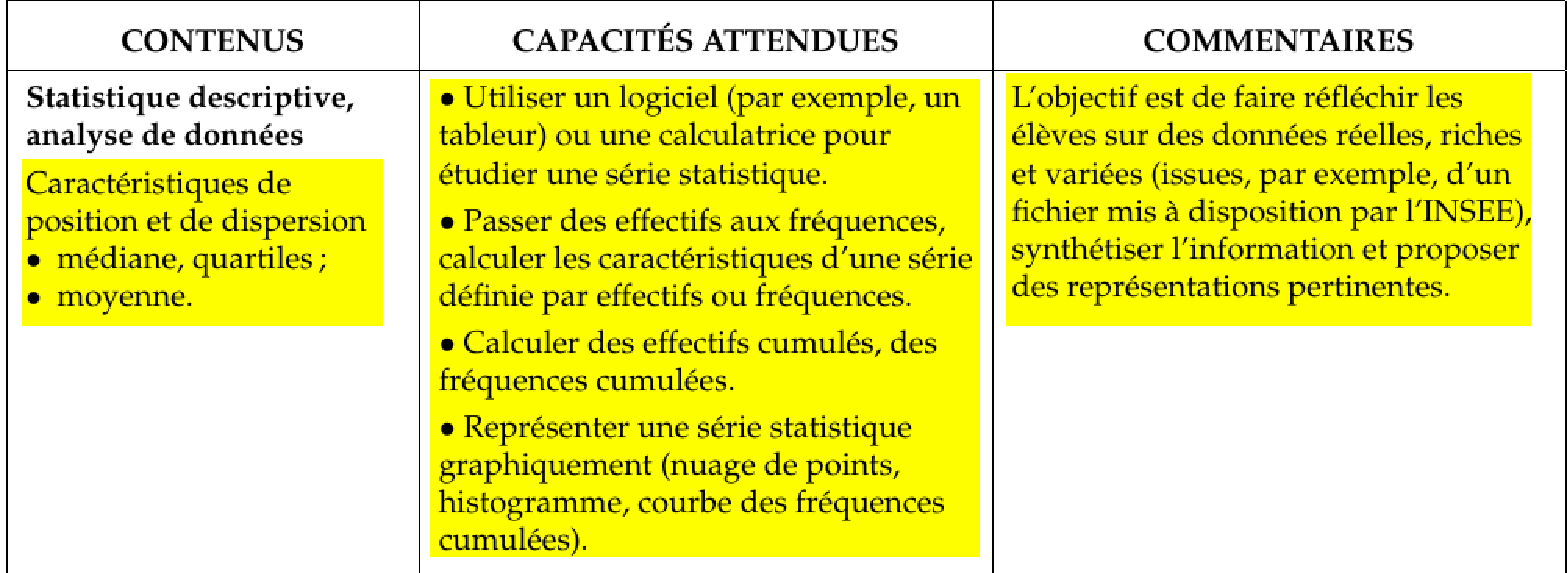
\includegraphics[width=\linewidth]{BO_statistique_descriptive}

\setcounter{section}{-1}
%+++++++++++++++++++++++++++++++++++++++++++++++++++++++++++++++++++++++++++++++++++++++++++++++++++++++++++++++++++++++++++ 
\section{Activité : un peu de spam ?}
%+++++++++++++++++++++++++++++++++++++++++++++++++++++++++++++++++++++++++++++++++++++++++++++++++++++++++++++++++++++++++++

% This is part of Un soupçon de mathématique sans être agressif pour autant
% Copyright (c) 2013
%   Laurent Claessens
% See the file fdl-1.3.txt for copying conditions.

% ATTENTION : les chiffres donnés ici sont repris dans le cours au moment des ECC.

\begin{wrapfigure}[5]{r}{8cm}
   \vspace{-0.5cm}        % à adapter.
   \centering
   \input{Fig_YRQOoPE.pstricks}
\end{wrapfigure}

Le graphique ci-contre illustre le nombre de spam reçus aujourd'hui par les élèves d'une classe.
\begin{enumerate}
    \item
        Combien d'élèves y-a-t-il dans la classe ?
    \item
        Combien d'élèves ont reçu \( 5\) spams ou plus ?
    \item
        En moyenne combien de spam ont reçu les élèves aujourd'hui ?
    \item
        Diviser la classe en 4 groupes suivant le nombre de spams reçus.
\end{enumerate}



Éléments de réponse.

\begin{enumerate}
    \item
Nous pouvons remplir le tableau
\begin{equation*}
    \begin{array}[]{|c||c|c|c|c|c|c|c|c|c|c|c|| c |}
        \hline
        \text{Nombre}&1&2&3&4&5&6&7&8&9&10&11&\text{total}\\
        \hline\hline
        \text{Effectifs}&3&0&1&4&4&2&1&5&3&1&1&25\\
        \hline
    \end{array}
\end{equation*}
\item
Il y a \( 17\) élèves ayant reçu \( 5\) spams ou plus.
     \item
         Pour calculer la moyenne il faut d'abord calculer le nombre total de spams reçus, puis diviser par le nombre d'élèves :
         \begin{equation}
             \text{moyenne}=\frac{ 3\times 1+1\times 3+4\times 4+4\times 5+2\times 6+\ldots+1\times 11 }{ 25 }=\frac{ 149 }{ 25 }=5.96.            
         \end{equation}
     \item
         En ce qui concerne la division de la classe en quatre groupe, vu que \( 25\) n'est pas divisible en \( 4\), il va falloir donner une convention sur les arrondis.
\end{enumerate}

%+++++++++++++++++++++++++++++++++++++++++++++++++++++++++++++++++++++++++++++++++++++++++++++++++++++++++++++++++++++++++++ 
\section{Les quartiles et la médiane}
%+++++++++++++++++++++++++++++++++++++++++++++++++++++++++++++++++++++++++++++++++++++++++++++++++++++++++++++++++++++++++++

\begin{definition}
    Nous considérons une liste de \( n\) valeurs triées par ordre croissant (avec éventuellement les répétitions).
    \begin{enumerate}
        \item
            La \defe{médiane}{médiane}, est la valeur qui sépare la liste en deux parties égales. C'est le terme du milieu si l'effectif total est impair et la moyenne des deux termes du milieu si l'effectif total est pair.
      \item 
          Le \defe{premier quartile}{quartile!premier} $Q_1$ est la plus petite valeur de la liste telle qu'au moins un quart des valeurs de la liste soient inférieures ou égales à $Q_1$.
        \item
            Le \defe{troisième quartile}{quartile!troisième} $Q_3$ est la plus petite valeur de la liste telle qu'au moins les trois quarts des valeurs de la liste soient inférieures ou égales à $Q_3$.
  \end{enumerate}
\end{definition}
En pratique :
\begin{itemize}
    \item 
  Pour le calcul de $Q_1$, on calcule $\dfrac{n}4$, puis on détermine le premier entier $p$ supérieur ou égal à $\dfrac{n}4$. Cet entier $p$ donne le rang de $Q_1$. 
  \item
  Pour le calcul de $Q_3$, on fait de même en remplaçant $\dfrac{n}4$ par $\dfrac{3n}4$. 
\end{itemize}


\begin{example}

    Un laboratoire expérimente un médicament sur dix souris. Voici les temps (en semaines) que les souris ont encore vécu après l'injection : \( 2\), \( 5\), \( 10\), \( 2\), \( 1\), \( 3\), \( 10\), \( 5\), \( 5\), \( 1\).

    D'abord nous trions par ordre croissant en respectant les répétitions :
    \begin{equation*}
        \begin{array}[]{|c||c|c|c|c|c|c|c|c|c|c|}
            \hline
            \text{numéro de la souris}&1&2&3&4&5&6&7&8&9&10\\
            \hline
            \text{semaines de vie}&1&1&2&2&3&5&5&5&10&10\\
            \hline
        \end{array}
    \end{equation*}

    Il y a \( 10\) valeurs, donc 
    \begin{enumerate}
        \item
            Pour le premier quartile, \( \frac{ 10 }{ 4 }\simeq 2.5\), on prend la troisième valeur : \( Q_1=2\).
        \item
            Pour le troisième quartile, \( \frac{ 3}{ 4 }\times 10\simeq 7.5\), on prend la huitième valeur : \( Q_3=5\).
        \item
            Pour la médiane, on prend la moyenne entre la cinquième et la sixième valeur : \( \frac{ 3+5 }{2}=4\) : \( Med=4\).
    \end{enumerate}

    Nous résumons ces informations sur le diagramme suivant :


    \begin{center}
        \input{Fig_DNYAefI.pstricks}
    \end{center}


    Attention : nouvelle de dernière minute. Le laboratoire s'est trompé dans ses résultats. En réalité les deux souris qui ont vécu \( 10\) semaines ont vécu respectivement \( 15\) et \( 20\) semaines. Est-ce que ça change quelque chose ?

\end{example}

Avec ces définitions de quartile et de médiane, nous avons la distribution suivante :

\begin{center}
   \input{Fig_KDtwIJf.pstricks}
\end{center}

\section{Représentation graphique d'une série statistique}

%--------------------------------------------------------------------------------------------------------------------------- 
\subsection{Effectifs cumulés croissants}
%---------------------------------------------------------------------------------------------------------------------------

Nous classons les élèves d'une classe d'après la première lettre de leur noms. Le résultat est le tableau
\begin{center}
\begin{tabular}[]{|c||c|c|c|c|c|c|c|c|c|c|c|c||c|}
        \hline
        Lettre&a&b&c&d&h&j&l&m&p&r&s&t&total\\
        \hline\hline
        Effectifs&4&8&9&2&2&1&1&2&2&1&1&2&35\\
        \hline
        ECC&4&12&21&23&25&26&27&29&31&32&33&35&\\
        \hline
\end{tabular}
\end{center}

\input{Fig_MAXkaGz.pstricks}

Reprenons l'exemple du spam
\begin{equation*}
    \begin{array}[]{|c||c|c|c|c|c|c|c|c|c|c|c|| c |}
        \hline
        \text{Nombre}&1&2&3&4&5&6&7&8&9&10&11&\text{total}\\
        \hline
        \text{Effectifs}&3&0&1&4&4&2&1&5&3&1&1&25\\
        \hline
        \text{ECC}&3&3&4&8&12&14&15&20&23&24&25&\\
        \hline
    \end{array}
\end{equation*}

\begin{Aretenir}
    \begin{enumerate}
        \item
            Les effectifs cumulés croissants s'obtiennent en additionnant successivement les effectifs.
        \item
            La différence des ordonnées entre deux points successifs du graphe des ECC donne l'effectif correspondant à l'abscisse du deuxième point.
    \end{enumerate}
\end{Aretenir}

%--------------------------------------------------------------------------------------------------------------------------- 
\subsection{Graphe des fréquences cumulées croissantes}
%---------------------------------------------------------------------------------------------------------------------------

\begin{definition}
    La \defe{fréquence}{fréquence} d'une valeur est le rapport
    \begin{equation}
        \frac{ \text{effectif de la valeur} }{ \text{effectif total} }.
    \end{equation}
\end{definition}

\begin{Aretenir}
    La fréquence est un nombre entre \( 0\) et \( 1\). Le zéro correspond à «personne» et le \( 1\) correspond à «tout le monde».
\end{Aretenir}

Nous reprenons l'exemple du spam
\begin{equation*}
    \begin{array}[]{|c||c|c|c|c|c|c|c|c|c|c|c|| c |}
        \hline
        \text{Nombre}&1&2&3&4&5&6&7&8&9&10&11&\text{total}\\
        \hline\hline
        \text{Effectifs}&3&0&1&4&4&2&1&5&3&1&1&25\\
        \hline
        \text{Fréquences}&\hphantom{0.001}&\hphantom{0.001}&\hphantom{0.001}&\hphantom{0.001}&\hphantom{0.001}&\hphantom{0.001}&\hphantom{0.001}&\hphantom{0.001}&\hphantom{0.001}&\hphantom{0.001}&\hphantom{0.001}&\hphantom{0.001}\\
        \hline
        \text{FCC}&&&&&&&&&&&&\\
        \hline
    \end{array}
\end{equation*}

Le résultat est :
\begin{equation*}
    \begin{array}[]{|c||c|c|c|c|c|c|c|c|c|c|c|| c |}
        \hline
        \text{Nombre}&1&2&3&4&5&6&7&8&9&10&11&\text{total}\\
        \hline\hline
        \text{Effectifs}&3&0&1&4&4&2&1&5&3&1&1&25\\
        \hline
        \text{Fréquences}&0.12&0&0.04&0.16&0.16&0.08&0.04&0.2&0.12&0.04&0.04&1\\
        \hline
        \text{FCC}&0.12&0.12&0.16&0.32&0.48&0.56&0.6&0.8&0.92&0.96&1&\\
        \hline
    \end{array}
\end{equation*}
Attention : le total risque de ne pas tomber sur \( 1\) à cause des arrondis faits un peu partout.

\begin{center}
\input{Fig_FWyrYhJ.pstricks}
\end{center}

\begin{remark}
    Le total des fréquences doit faire \( 1\). Le dernier point du graphe des fréquence cumulées croissantes est donc d'ordonnée \( 1\).

    Des erreurs d'arrondis dans dans le calcul des fréquences peuvent entrainer que la somme ne vaut pas \( 1\).

    En pratique, pour dessiner le graphe des FCC il vaut mieux calculer les ECC puis les fréquences correspondantes, et non les fréquences et additionner.

\end{remark}

%--------------------------------------------------------------------------------------------------------------------------- 
\subsection{Histogramme}
%---------------------------------------------------------------------------------------------------------------------------

%TODO : c'est mieux de ne pas parler d'histogrammes à pas constant, mais directement de pas non constant et de montrer un exemple  qui tombe bien sur le quadrillage.

%///////////////////////////////////////////////////////////////////////////////////////////////////////////////////////////
\subsubsection{Le problème}
%///////////////////////////////////////////////////////////////////////////////////////////////////////////////////////////

Si nous regardons le chiffre d'affaire d'entreprises, il y a peu de chances que l'effectif de entreprises dont le chiffre d'affaire est exactement \( 14.258.736\)€ soit grand. Supposons avoir les nombres
\begin{center}
    100,101,105,502,503.
\end{center}
Il est immédiatement visible qu'il y a un paquet autour entre \( 100\) et \( 200\) et un paquet autour entre \( 500\) et \( 600\)a. Pourtant tracer le graphe des effectifs n'est pas très instructif :
\begin{center}
   \input{Fig_JXWXdJI.pstricks}
\end{center}

%///////////////////////////////////////////////////////////////////////////////////////////////////////////////////////////
\subsubsection{La solution}
%///////////////////////////////////////////////////////////////////////////////////////////////////////////////////////////

Nous regroupons les entreprises en classes d'entreprises «semblables». Par exemple :
\begin{itemize}
    \item Les entreprises de CA entre 100 et 200. Effectif : 3.
    \item Les entreprises de CA entre 200 et 300. Effectif : 0.
    \item Les entreprises de CA entre 300 et 400. Effectif : 0.
    \item Les entreprises de CA entre 400 et 500. Effectif : 0.
    \item Les entreprises de CA entre 500 et 600. Effectif : 2.
\end{itemize}

Le graphe de ces classe ressemble à :
\begin{center}
   \input{Fig_PUGmLBC.pstricks}
\end{center}
Là, les choses sont déjà plus claires.

%--------------------------------------------------------------------------------------------------------------------------- 
\subsection{Exemple}
%---------------------------------------------------------------------------------------------------------------------------

Le tableau suivant donne la répartition des entreprises du secteur automobile en fonction de leur chiffre d'affaire (en millions d'euros).

\begin{center}
    \begin{tabular}{|c||c|c|c|c|c|c|}
        \hline
        chiffre d'affaire&moins de \( 0.25\)&\( \mathopen[ 0.25 ,0.5 [\)&$\mathopen[ 0.5;1  [$&$\mathopen[ 1 , 2.5 [$&$\mathopen[ 2.5;5 ,  [$&$\mathopen[ 5 , 10 [$\\
            \hline\hline
            nombre d'entreprises&\( 137\)&\( 106\)&\( 112\)&$154$&\( 100\)&\( 33\)\\
            \hline
    \end{tabular}
\end{center}

\begin{Aretenir}
Pour des données rassemblées en classes, l'\textbf{aire} du rectangle est proportionnelle à l'effectif (ou à la fréquence). 
\end{Aretenir}

Nous en dessinons l'histogramme suivant :
\begin{center}
   \input{Fig_LTenBUj.pstricks}
\end{center}


Consignes pour dessiner un histogramme :
\begin{enumerate}
    \item
        Trouver la plus haute boîte en calculant le rapport \( \frac{ \text{effectif} }{ \text{largeur} }\) pour chaque boîte.
    \item
        Se fixer une échelle pour que la plus haute boîte reste raisonnable : elle ne doit pas faire deux mètres de haut, ni un centimètre. Il faut viser environ \unit{10}{\centi\meter}.
    \item
        Tracer les boîtes.
    \item
        Mettre la graduation \emph{horizontale} en écrivant la légende correspondante.
    \item
        Ne pas mettre de graduation verticale en cas d'histogramme à pas non constant\footnote{C'est à dire ceux dont la largeur n'est pas la même pour toute les boîtes.}.
    \item
        Écrire l'effectif de la boîte au-dessus de la boîte.
    \item
        Éventuellement écrire l'unité de surface «un carreau= \ldots effectifs». Par exemple «un carreau = 50 entreprises», «un carreau = 15 personnes».
\end{enumerate}

%\begin{example}
%    Si nous avons un effectif de \( 25\) personnes, un quart des effectifs seraient \( 6.25\) personnes, et les trois quarts seraient \( 18.75\) personnes. Donc nous mettons les premier quartile sur la \( 7\Ieme\) personne et le troisième quartile sur la \( 19\Ieme\) personne.

%    Le premier quart des effectifs seraient donc les personnes numéro \( 1\), \( 2\), \( 3\), \( 4\), \( 5\), \( 6\) et \( 7\). Et le dernier quart des personnes seront les personnes numéro \( 20\), \( 21\), \( 22\), \( 23\), \( 24\) et \( 25\).
%\end{example}

%+++++++++++++++++++++++++++++++++++++++++++++++++++++++++++++++++++++++++++++++++++++++++++++++++++++++++++++++++++++++++++ 
\section{Distribution de DS}
%+++++++++++++++++++++++++++++++++++++++++++++++++++++++++++++++++++++++++++++++++++++++++++++++++++++++++++++++++++++++++++

Voici quelque exemples de diagrammes en boîtes pour les DS.

Pour une des secondes :
\begin{center}
   \input{Fig_PEoyeQt.pstricks}
\end{center}

Et pour l'autre :
\begin{center}
   \input{Fig_GSfDCyx.pstricks}
\end{center}
